 
\documentclass[12pt,a4paper]{article}
\usepackage[utf8x]{inputenc}
\usepackage[english, spanish]{babel}
\setlength{\parskip}{0.8em}
\usepackage{url}
\usepackage{graphicx}

\usepackage{bookmark}
\usepackage{natbib}
\usepackage{csquotes}
\usepackage{wrapfig}
\usepackage{amsmath}
\usepackage{mathtools}
\usepackage{amsfonts}
\usepackage{amssymb}
\usepackage{graphicx}

\usepackage[font=small,format=plain,labelfont=bf,up,textfont=it,up]{caption}
\usepackage{diagbox}
\providecommand{\abs}[1]{\lvert#1\rvert}
\newcommand{\grad}{^{\circ}}
\usepackage[makeroom]{cancel}
\usepackage{enumitem}
\usepackage{float}	
\usepackage{setspace}
\usepackage{subfigure}
\usepackage[export]{adjustbox}
\usepackage{booktabs}
\usepackage{bigstrut}
\usepackage{multirow}
\usepackage{array}
\usepackage{tabularx}
\usepackage{lipsum}  
\usepackage{sectsty}
\usepackage{titlesec}
\usepackage{verbatim}

\usepackage{lscape}
\usepackage{tabu}
\usepackage{array}
\newcolumntype{P}[1]{>{\centering\arraybackslash}p{#1}}
\usepackage{xcolor}
\definecolor{dark}{rgb}{0.10,0.2,0.3}
\definecolor{seablue}{rgb}{0.10,0.2,0.45}
\definecolor{light}{rgb}{1.7,1.5,0.6}
\definecolor{purpure}{rgb}{0.5,0.15,0.3}
\definecolor{bluegreen}{rgb}{0.2,0.65,0.65}
\definecolor{bluegreen2}{rgb}{0.2,0.45,0.45}
\definecolor{vcromo}{rgb}{0.0,0.18,0.39}
\usepackage{hyperref}
\hypersetup{colorlinks,%
citecolor=dark,%
filecolor=dark,%
linkcolor=bluegreen,%
urlcolor=purpure}

%%%%% FOR CODE IN LATEX %%%%

\usepackage{listing}
\usepackage{listings}
\usepackage{minted}

\usepackage{kvoptions}
\usepackage{fancyvrb}
\usepackage{fvextra}	
\usepackage{upquote}
\usepackage{float}
\usepackage{ifthen}
\usepackage{calc}
\usepackage{ifplatform}
\usepackage{etoolbox}
\usepackage{pdftexcmds}
\usepackage{xstring}
\usepackage{lineno}
\usepackage{framed}



\definecolor{codegreen}{rgb}{0,0.5,0}
\definecolor{codegray}{rgb}{0.5,0.5,0.5}
\definecolor{codepurple}{rgb}{0.58,0,0.82}
\definecolor{backcolour}{rgb}{0.95,0.95,0.92}

\lstdefinestyle{mystyle}{
    backgroundcolor=\color{white},   
    commentstyle=\color{codegreen},
    keywordstyle=\color{blue},
    numberstyle=\tiny\color{codegray},
    stringstyle=\color{codepurple},
    basicstyle=\ttfamily\footnotesize,
    breakatwhitespace=false,         
    breaklines=true,                 
    captionpos=b,                    
    keepspaces=true,                 
    numbers=left,                    
    numbersep=5pt,                  
    showspaces=false,                
    showstringspaces=false,
    showtabs=false,                  
    tabsize=2
}


%%%%%%%%
\usepackage[left=3cm,right=3cm,top=2.5cm,bottom=2.5cm]{geometry}

% \titleformat{\section}
%  {\normalfont\sffamily\bfseries\Large\color{vcromo}}
%   {\thesection}{1em}
%   {\sectionrule{25pt}{0.8pt}{-12pt}{0.8pt}}
  
\titleformat{\section}[frame]
{\normalfont\sffamily\bfseries\Large\color{vcromo}}{}
{10pt}{\LARGE\bfseries\filcenter}

  
\titleformat{\subsection}
  {\normalfont\itshape\large\bfseries\color{dark}}
  {\thesubsection}{1em}{}



\setcounter{secnumdepth}{5}
\setcounter{tocdepth}{5}

\providecommand{\abs}[1]{\lvert#1\rvert}
\providecommand{\norm}[1]{\lVert#1\rVert}


\begin{document}
%------Portada--------------%
	\begin{titlepage}
	\centering
    {
\includegraphics[width=0.3\textwidth]{fotos/Logo_azul.png}\par}
	\vspace{1cm}
	{\bfseries\LARGE Universidad Politécnica de Madrid \par}
	\vspace{0.3cm}
	{\scshape\Large Escuela Técnica Superior de Ingenieros Industriales \par}
	\vspace{2.5cm}
	{\scshape\Huge Programación de Sistemas \par}
	\vspace{0.3cm}
	{\scshape\large Departamento de Electrónica y Automática \par}
	\vspace{2cm}
    {\itshape\LARGE Práctica 2: Programación de un videojuego \par}
    \vspace{0.5cm}
    {\upshape\large Programación en ANSI C++ de una \emph{lista enlazada} (ObjectList) para la gestión de un videojuego (estilo \textit{Asteroids})}
	\vfill
	{\large{Celia \textsc{Ramos Ramírez} (18295)\par}}
	\vspace{0.1cm}
    {\large{Gonzalo \textsc{Quirós Torres} (17353)\par}}
	\vspace{0.1cm}
	{\large{Josep María \textsc{Barberá Civera} (17048)\par}}
	\vfill
	{\Large{ $3\grad$ \textsc{GITI}}\par}
	\vfill
	{\Large \today \par}
	\end{titlepage}
	
%-----Página en blanco------%
% \newpage
% \begin{center}
% \textit{\{Esta página se ha dejado intencionadamente en blanco\}}
% \end{center}
% \thispagestyle{empty} %	
% \newpage

%%%%%%%%%%%%%%%%%%%%%%%%%%%%%%%%%%%%%%%%%%%%%
%%%%%%%%%%%%%%%%% RESUMEN %%%%%%%%%%%%%%%%%%%
%%%%%%%%%%%%%%%%%%%%%%%%%%%%%%%%%%%%%%%%%%%%%

\section*{Resumen}
 

%%%%%%%%%%%%%%%%%%%%%%%%%%%%%%%%%%%%%%%%%%%%%
%%%%%%%%%%%%%%%%% ÍNDICE %%%%%%%%%%%%%%%%%%%%
%%%%%%%%%%%%%%%%%%%%%%%%%%%%%%%%%%%%%%%%%%%%%

{
 \setlength{\parskip}{0.2em}
 \hypersetup{linkcolor=black}
 %Fijaros que estoy cambiando el color solo localmente...es genial para mantener los liks pero que no sea muy cargante el color para el índice de contenidos!!!
 \tableofcontents
}
% \pagenumbering{Roman}

%Si quieres que aparezca en el indice de contenidos pero sin numeración, poner lo siguiente simpre después de algún apartado
%\phantomsection
%\addcontentsline{toc}{subsection}{Manolo el del bombo}

%%%%%%%%%%%%%%%%%%%%%%%%%%%%%%%%%%%%%%%%%%%%%
%%%%%%%%%%%%%% INTRODUCCIÓN %%%%%%%%%%%%%%%%%
%%%%%%%%%%%%%%%%%%%%%%%%%%%%%%%%%%%%%%%%%%%%%

\section{Introducción}

En esta memoria se presenta una posible implementación en ANSI C++ para gestionar un videojuego estilo \emph{Asteroids} mediante el uso de la librería gráfica multi-plataforma \textsc{OpenGL}.

El entorno de programación utilizado ha sido \textsc{Visual Studio Code}. Se ha gestionado el trabajo mediante el uso de GitHub y la extensión \emph{Live Share} que ofrece VSCode.

El videojuego elegido es el famoso juego arcade \emph{Asteroids} de Atari de 1979 \cite{wiki}. Se han implementado las clases con sus atributos y métodos necesarios así como la lógica del juego para su correcto funcionamiento.
Los requisitos cubiertos a grandes rasgos han sido:
\begin{itemize}
    \item Creación de una clase \emph{ObjectList} que gestiona una lista enlazada de los objetos del juego.
    \item Creación de la clase Alien, necesaria para instanciar el objeto \emph{theUFO}.
    \item Integración del Ovni en la lógica del juego.
    \item Ajuste del sistema de puntuaciones.
\end{itemize}

Además de estos requisitos, se ha implementado alguna característica extra como que de un Ovni aparezca otro algunas veces cuando este sea destruido, o una nueva clase llamada \#angel\# que otorga vidas al ser capturado por la nave. Dichos extras otorgan emoción al juego.


%%%%%%%%%%%%%%%%%%%%%%%%%%%%%%%%%%%%%%%%%%%%%
%%%%%%%%%%%%%% DIAGRAMAS %%%%%%%%%%%%%%%%%%%%
%%%%%%%%%%%%%%%%%%%%%%%%%%%%%%%%%%%%%%%%%%%%%

\section{Diagramas}
\subsection{Diagramas de Clases (UML)}
Para entender correctamente la relación entre las clases, tanto de las ya dadas en el fichero original como de las creadas posteriormente, se ha realizado un diagrama de clases en formato \emph{UML} para ello se ha empleado el programa StarUML\textsuperscript{\textregistered}.

\begin{figure}[h]
    \centering
    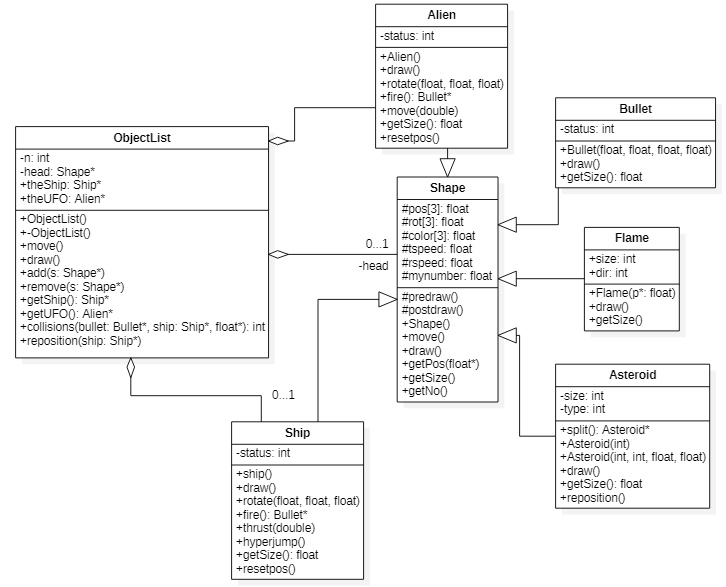
\includegraphics[width=\textwidth]{fotos/UML.PNG}
    \caption{Diagrama de clases del juego mediante \emph{StarUML}}
    \label{uml}
\end{figure}

Como puede verse en la Ilustración \ref{uml}, la clase \emph{ObjectList} agrega punteros a las clases \emph{Alien}, \emph{Ship} y \emph{Angel}, además de contener un puntero tipo \emph{Shape} llamado \textit{head} que apunta a la cabeza de la lista (pero que en la implementación realizado no se utiliza). Al igual que la clase \emph{Ship}, las clases \emph{Alien}, \emph{Angel}, \emph{Bullet}, \emph{Flame} y \emph{Asteroid} son hijas de la clase \emph{Shape}. La clase \emph{Alien} tiene mucho en común con la clase \emph{Ship}, pues realizan prácticamente lo mismo, con la diferencia de que el OVNI (instancia de la clase \emph{Alien}) se mueve automáticamente y de forma errática sin ser necesaria la interacción con el usuario. Por comodidad se han añadido dos punteros, uno al OVNI y otro a la astronave (\emph{theShip}), que simplificarán mucho el código tanto en la lógica del juego como en la implementación de la clase \emph{ObjectList}.
A parte de las clases aquí representadas, existe otro archivo de cabecera llamado \emph{commonstuff}, que almacena funciones cortas, parámetros y llamadas a librerías usadas en todos los archivos fuente del programa.
\subsection{Diagramas de comunicación}

El siguiente diagrama ilustra desde dónde se crean los objetos que se van a usar en el resto del programa:

\begin{figure}[h]
    \centering
    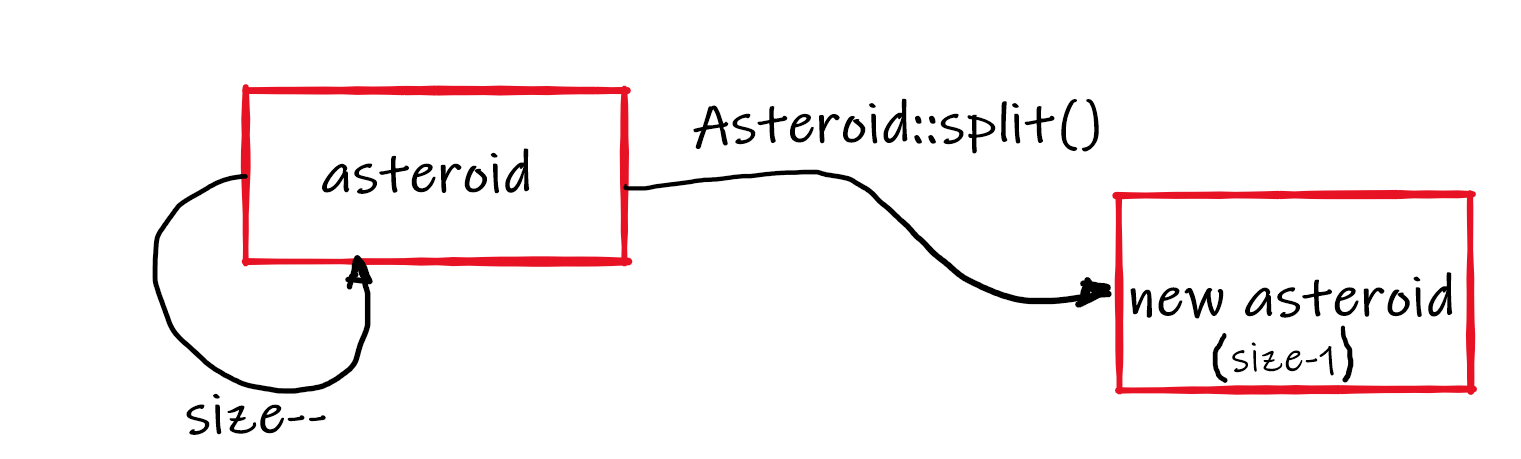
\includegraphics[width=\textwidth]{fotos/asteroid.png}
    \caption{Diagrama de comunicación }
    \label{asteroid}
\end{figure}

El diagrama de la Ilustración \ref{asteroid} representa el mecanismo de creación de los objetos más importantes que se lleva a cabo en el constructor del objeto \emph{ObjectList} y la creación de la bala a través del método \textsc{fire()} del objeto \emph{theShip}. Se crean también todos los asteroides, donde su número concreto viene definido por el parámetro \textsc{NUMASTEROIDS} definido en \emph{commonstuff.hpp}. Los asteroides son inmediatamente cargados en la interfaz gráfica mediante la función $push_front()$ de la plantilla $<list>$, a diferencia del OVNI (\emph{theUFO}), que será cargado desde la lógica del juego cuando se cumplan las condiciones especificadas en el algoritmo.
A continuación, en otro pequeño diagrama de objetos, se verá el comportamiento de uno de los objetos \emph{Asteroid} cuando es impactado por una bala o por la astronave.


%%%%%%%%%%%%%%%%%%%%%%%%%%%%%%%%%%%%%%%%%%%%%
%%%%%%%%%% DESCRIPCION FUNCIONES %%%%%%%%%%%%
%%%%%%%%%%%%%%%%%%%%%%%%%%%%%%%%%%%%%%%%%%%%%

\section{Descripción de funciones y estructuras del juego}
\subsection{Clase ObjectList}

La clase \emph{ObjectList} hereda características de la plantilla {\textless list\textgreater} lo que permite implementar de forma muy sencilla una lista enlazada. Esta lista enlazada es necesaria para gestionar todos los objetos que han sido creados en el constructor del objeto \emph{ObjectList} de forma eficiente. 
Por un lado, esta clase declara los objetos que serán usados durante el resto del programa y también realiza algunas funciones básicas como son eliminar estos objetos, moverlos o dibujarlos.

Además de declarar los objetos, la clase \emph{OjectList} también hace visibles objetos ya creados mediante su función \textsc{add()}, que será muy útil para hacer visible el \emph{ovni} cuando tenga que aparecer y hacer visibles los nuevos asteroides creados fruto de una colisión. 
Por comodidad, en la propia clase se han implementado dos métodos que devuelven un puntero a la \emph{nave} y al \emph{ovni}: \textsc{getShip()} y \textsc{getUFO()}, respectivamente. Estos punteros permitirán acceder a los métodos de ambas clases más fácilmente que si no estuvieran implementados.

Por otro lado, la función principal de la clase ObjectList es la función collisions() que devuelve entero. El entero devuelto permitirá identificar al tipo de colisión que se ha producido y permitirá a la lógica del programa, implementada en el archivo fuente mainAsteroids.cpp, gestionar las puntuaciones y eliminar o añadir objetos cuando proceda. En primer lugar, la función asigna tamaños y posiciones de los objetos principales esto es la nave, el ovni y la bala. posteriormente comprueban las distancias entre algunos de estos objetos susceptibles de colisionar, esto es: asteroides y astronave, asteroides y bala, OVNI y bala y astronave y ovnis.

\begin{itemize}
    \item En el primer caso, el choque entre un asteroide y la astronave, el asteroide se divide o se destruye dependiendo de su tamaño y la astronave se destruye y si no era la última, una nueva astronave se reposiciona en el centro.
    \item Cuando una bala choca con un asteroide el asteroide se divide o se destruye dependiendo de su tamaño y la bala se destruye.
    \item Cuando la bala choca con el ovni tanto el ovni como la bala se destruyen, aunque puede ocurrir que donde había un ovni inmediatamente surja otro no ocurre todas las veces y el comportamiento es aleatorio.
    \item Cuando una astronave choca con un ovni o viceversa, el ovni queda intacto pero la astronave se destruye reposicionándose en el centro si todavía quedan vidas y si no es así se termina el juego.
\end{itemize}

En cada nueva llamada a la función \textsc{collisions()} se comprueban todos y cada uno de los elementos de la lista enlazada, obteniéndose sus posiciones y sus tamaños mediante un bucle \textsc{for()}. Dentro del bucle se obvian tanto la bala como la astronave pues se pasan como parámetros a la llamada de la función \textsc{collisions()} y no es necesario volver a comprobarlo, si bien es cierto que si se tienen en cuenta a la hora de comprobar las distancias entre los elementos que se han mencionado anteriormente. La comprobación de las distancias se hace mediante la función \textsc{mydistance()} definida en \emph{commonstuff.hpp}.

En todos los casos, cuando se detecta una colisión, se retorna un entero que indica el tipo de colisión y entre qué elementos se ha producido. Dependiendo del entero se actualiza la puntuación del jugador.  Además, en un vector dedicado a tal efecto se marcan las coordenadas de la explosión. La duración de la explosión será definida en la lógica del juego.

Otra función muy importante, la función \textsc{reposition()}, se encarga de reposicionar la nave cuando esta es destruida. También se encarga de reposicionar los asteroides cuando la reposición de la nave en el centro no es posible.

\subsection{Clase Alien}
La clase Alien hereda características de la clase Shape, lo que le otorga características muy similares al resto de figuras del juego. Esto facilita la integración con el resto del código, pues su tratamiento es muy similar al resto de figuras, aunque tiene características propias que son tratadas específicamente. La clase Alien comparte muchas similitudes con la clase Ship en cuanto a estructuración, pero su movimiento se imprime automáticamente desde un generador aleatorio de direcciones en la lógica del juego. Para que su movimiento sea autónomo es necesario llamar al método Alien::run() desde el método Alien::draw()

%%%%%%%%%%%%%%%%%%%%%%%%%%%%%%%%%%%%%%%%%%%%%
%%%%%%%%%%%%%%%%% PRUEBAS %%%%%%%%%%%%%%%%%%%
%%%%%%%%%%%%%%%%%%%%%%%%%%%%%%%%%%%%%%%%%%%%%

\section{Pruebas}


%%%%%%%%%%%%%%%%%%%%%%%%%%%%%%%%%%%%%%%%%%%%%
%%%%%%%%%%%%%%%% GUÍA DE USO %%%%%%%%%%%%%%%%
%%%%%%%%%%%%%%%%%%%%%%%%%%%%%%%%%%%%%%%%%%%%%

\section{Guía de uso}


%%%%%%%%%%%%%%%%%%%%%%%%%%%%%%%%%%%%%%%%%%%%%
%%%%%%%%%% REPARTO DE ROLES %%%%%%%%%%%%%%%%%
%%%%%%%%%%%%%%%%%%%%%%%%%%%%%%%%%%%%%%%%%%%%%

\section{Reparto de Roles}
Para el reparto de tareas se decidió seguir el mismo proceso que para el trabajo anterior. En los primeros pasos de la investigación se realizaron reuniones y recopilación de ideas en las cuales cada integrante del grupo desarrolló poco a poco un boceto de la clase \emph{ObjectList}.

Una vez se consiguió implementar dicha clase, se repartieron las tareas de desarrollo del resto del código entre Linux y Windows para seguir elaborando el programa y realizar pruebas en ambos sistemas operativos. 

Al mismo tiempo se realizaba el diseño de los diagramas UML que servía de apoyo para escribir los códigos de los elementos que conforman el juego.

Cuando se consiguió una versión funcional se repartieron entre el equipo tareas de optimización y solución de errores.

Finalmente, con el programa finalizado, surgió la idea de implementar una nueva clase para añadir un toque original al proyecto. Dos integrantes desarrollaron e implementaron la nueva adición mientras el tercero se ocupaba de la parte documentativa del proyecto. Mientras se manteniendo al día la memoria y se redactaba las descripciones necesarias acerca de este. 

%%%%%%%%%%%%%%%%%%%%%%%%%%%%%%%%%%%%%%%%%%%%%
%%%%%%%%% PROPUESTAS DE MEJORA %%%%%%%%%%%%%%
%%%%%%%%%%%%%%%%%%%%%%%%%%%%%%%%%%%%%%%%%%%%%

\section{Propuestas de mejora y valoración personal}
Al tener un carácter clásico, el juego resulta sencillo y en ello reside su gracia. Evidentemente, hay infinidad de mejoras o extensiones que se podrían implementar. Sin embargo la principal preocupación del equipo era conseguir la versión básica del juego funcionando para familiarizarse con el entorno de \textsc{OpenGL} y posteriormente, si se tenía el tiempo necesario, se implementaría alguna mejora.

Una vez conseguido el juego en su versión básica como se ha mencionado con anterioridad, a excepción del disparo del \emph{ovni} en dirección a la \emph{nave}. Se decide incorporar un \emph{power up} que recide el nombre de \emph{Angel} en el juego. Este nuevo elemento se trata de una tetera predefinida en \emph{OpenGL} que aparece después de 40 segundos de juego para otorgar al jugador la posibilidad de conseguir una vida extra si se acerca a ella y la ‘recoge’.


% \clearpage
\bibliographystyle{abbrv}
\bibliography{mybib}

\end{document}

